%!TEX root = ../report.tex

\begin{document}
    \chapter{Introduction}

    The development of Deep Neural Networks (DNNs) made tasks such as object classification \cite{alexnet} and object detection \cite{fasterrcnn}, \cite{fastrcnn} easy to solve.
    These DNNs have been deployed in various real-world scenarios such as autonomous driving \cite{autonomousdriving}, semi-autonomous robotic surgery \cite{roboticsurgery} and also in space rovers \cite{Marsrover_1}, \cite{Marsrover_2}.
    DNNs are majorly deployed in the perception stack in the autonomous driving pipeline. 
    Figure~\ref{fig:Apollopipeline} depicts the pipeline of the modules present in one of the open-source autonomous driving platforms called Apollo \cite{baiduapollo}.
    From this pipeline, one can infer that most of the decisions from the autonomous car's prediction and motion planning modules depend on the perception module's output.
    Since the perception module plays such significance, the developers of the perception stack must make sure the outputs are meaningful.
\begin{figure}[h!]
    \centering
    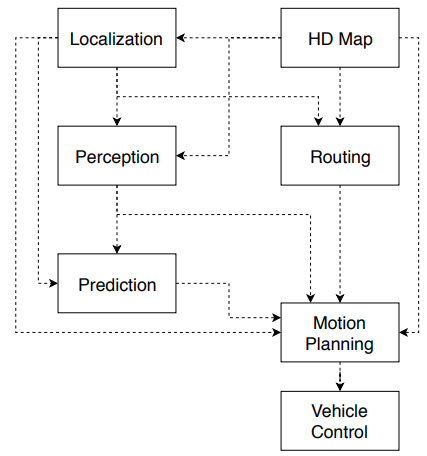
\includegraphics[scale=0.35]{images/Apollopipeline.png}
    \caption{Module pipeline for Apollo autonomous driving platform. Image taken from \cite{baiduapollo}}
    \label{fig:Apollopipeline}
\end{figure}

The DNNs utilized in the perception module need to be trained on the dataset, which should be similar to its deployment area.
For example, an autonomous driving agent must be trained on a dataset containing roads, vehicles, vegetation and other objects found around the road.
This closedness of the dataset, i.e., a fixed number of classes, will cause an issue when the DNN encounter an unknown object in the real world.
This unknown object will be predicted as one of the classes in the dataset, leading to radical decisions when this error is propagated down the pipeline in Figure \ref{fig:Apollopipeline}.
These unknown objects in the real world which are not present in the training dataset can be regarded as Out-of-Distribution (OOD) objects and the trained dataset is called In Distribution (ID) dataset. 
More discussion on the OOD is presented in Section~\ref{sec:oodvanom}.
The Tesla autonomous driving platform encounters one such problem of misdetection of unknown objects.
\begin{figure}[h!]
    \begin{subfigure}{0.48\textwidth}
        \centering
        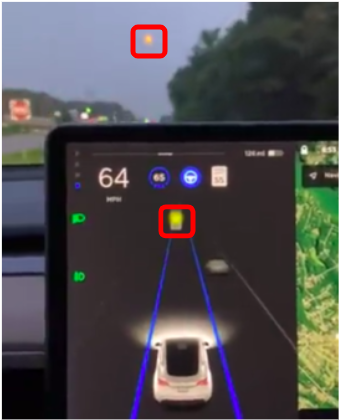
\includegraphics[scale=0.5]{images/tesla_1.png}
        \caption{}
        \label{fig:teslafails_1}
    \end{subfigure}
    \begin{subfigure}{0.48\textwidth}
        \centering
        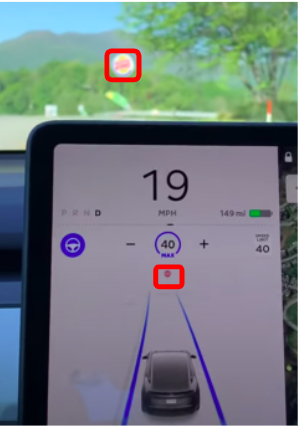
\includegraphics[scale=0.5]{images/tesla_2.png}
        \caption{}
        \label{fig:teslafails_2}
    \end{subfigure}
    \caption{Misdetection of OOD objects in Tesla autonomous driving platform. (a) Moon is detected as yellow signal light and (b) depicts the misdetection of Burger King sign as stop traffic sign. Images taken from \cite{tesla_fails}.}
\end{figure}

Figure~\ref{fig:teslafails_1} and Figure~\ref{fig:teslafails_2} depict the misdetections from the Tesla autonomous driving system.
The problem in the first image is that the moon is detected as the yellow signal light.
The second image has the problem of misdetection of the Burger King sign as a stop signal. 
These misdetections question the safety of the Deep Neural Networks (DNNs) predictions.
This thesis made an effort to detect these unknown objects in 3D LiDAR data using uncertainty scores for the task of 3D semantic segmentation.
We use the fact that the DNN predictions of unknown objects will have higher uncertain values.
A detailed discussion on types of uncertainty and what type of uncertainty can be used for OOD detection is discussed in Section~\ref{sec:ue_methods}.
Further in this chapter, we will discuss the task of 3D semantic segmentation, the problem statement and concludes with the contributions of this thesis.

\section{3D Semantic Segmentation}
Semantic segmentation is an important task in computer vision.
This is because of its widespread use in scene understanding which further helps in navigation and planning for autonomous robots.
The objective in semantic segmentation is to assign each point in the point cloud (each pixel in case of an image) a specific class.
In recent years, works such as \cite{spatialpyramidpool}, \cite{deeplabv3} and \cite{fcn} studied the task of semantic segmentation for images and has made advancements in terms of performance.
But with the limitations caused in images by uneven illumination and occlusion are a problem for semantic segmentation.
So researchers have turned towards alternatives like 3D point cloud or RGBD image.
In this thesis, we chose to utilize 3D point cloud generated from 3D LiDAR becuase, point clouds are unsuceptible to illumination and provides rich geometric information of a scene.
Typically, a point in the 3D point cloud is represented using spatial coordinates (XYZ) and along with the spatial information, other features such as colour (RGB), intensity and surface normals are also utilized.
Figure~\ref{fig:sem3d_gt_vis} represents the point cloud of a street scene collected from a 3D LiDAR and its respective semantic map.
Because of the above advantages with the 3D point cloud, LiDAR has been one of the central component in the sensor suite for SLAM systems in robotic applications \cite{thrun2006stanley}, \cite{patz2008practical}, \cite{hess20162dSLAM} and autonomous driving \cite{li2016vehicle}.
Also to the best of our knowledge current State-Of-The-Art (SOTA) 3D semantic segmentation models were developed to use 3D point cloud data, and these SOTA models were studied in this thesis and discussed in Section~\ref{sec:dl_approach}.

\section{Problem Statement}
This thesis studies OOD detection over the task of 3D semantic segmentation.
Notably, we study the 3D semantic segmentation datasets available and create a benchmark for the ID and OOD datasets.
Similar to \cite{Cao}, we define the OOD data based on two categories.
In the first case, we define a point in the point cloud as OOD if the point is from an unknown class which is not present in the training set.
As an example, \cite{liang2017enhancing_ODIN} uses CIFAR-10 vs SVHN. Where CIFAR-10 consits of outdoor objects like airplane, automobile and SVHN consist of images with digits.
In the second category, we define a point in the point cloud as OOD if the features of the point are of inferior quality.
An example for this category, can be LiDAR data collected on a foggy day, as fog causes noise in the data.


The other major issue we address in this thesis is the OOD detection methods. 
Existing OOD detection methods are tested for 2D classification and 2D semantic segmentation tasks, and the applicability of
these methods to 3D semantic segmentation tasks is not studied. Moreover, the proposed OOD detection
techniques are evaluated on simple datasets. The performance of these methods on complex and
feature-rich 3D datasets is questionable. Additionally, the high dimensionality of the 3D data imposes computational constraints. In recent years, uncertainty estimation has gained prominence. Past works
indicate that uncertainty is also an effective tool in detecting OOD (in the 2D domain). So we also research
whether uncertainty estimation is a practical approach for OOD detection in the 3D domain.
% \newline
% 
% The research questions answered by this thesis are:
% \begin{itemize}
%     \item[\textbf{R1}] How to create a benchmark over 3D segmentation datasets for the OOD setting?, i.e., create the in-distribution and out-distribution datasets.
%     \item[\textbf{R2}] Are current OOD detection methods developed and evaluated for 2D tasks, effective in 3D domain?
%     \item[\textbf{R3}] Is uncertainty quantification an effective approach to classify OOD detection in 3D semantic segmentation models?
%     % \item[\textbf{R4}] What metrics can be applied for the OOD detection task over 3D semantic segmentation models? 
%     \item[\textbf{R4}] How to evaluate the OOD detections over the 3D semantic segmentation task?
% \end{itemize}

\section{Contributions}
The contributions made in this thesis are
\begin{enumerate}
    \item A complete survey of the available 3D LiDAR datasets and 3D semantic segmentation models.
    \item Benchmarking of 3D LiDAR datasets for OOD detection. We proposed two benchmark datasets Sematic3D vs S3DIS and Semantic3D vs Semantic3D without colour, with Semantic3D being In-Distribution (ID) dataset, S3DIS and Semantic3D without colour being Out-Of-Distribution (OOD) datasets.
    \item A survey on the uncertainty estimation methods and classical OOD methods.
    \item An evaluation of OOD detection on benchmarked datasets over the RandLA-Net model using Deep Ensembles and Flipout.
\end{enumerate}

To summarize this chapter, we discussed the motivation behind the problem of OOD detection, like
how errors in perception module results lead to catastrophic consequences in an autonomous driving pipeline.
We also discussed this problem in a real world example of Tesla autonomous driving platform.
This is followed by discussion on 3D semantic segmentation and LiDAR point clouds.
Finally, we discussed the problem statement and concluded with the contributions of this thesis.
The following chapters include the study of the state-of-the-art, experimentation details like methodology and setup, results and conclusion chapters.


%\begin{figure}[h!]
%    \begin{subfigure}{0.333\textwidth}
%        \centering
%        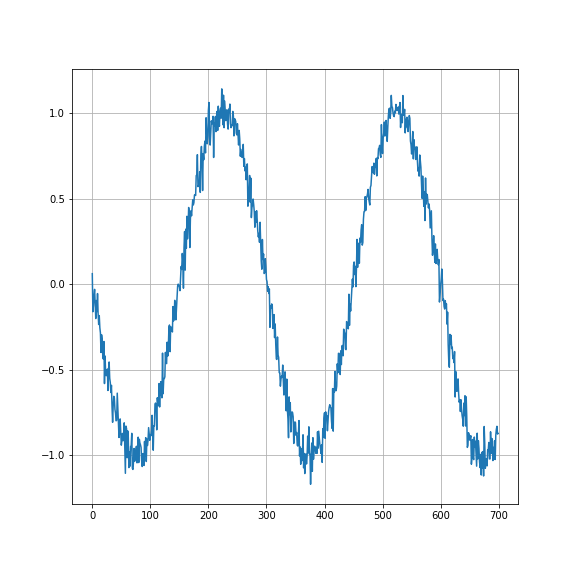
\includegraphics[height=0.3\textheight,width=0.98\textwidth]{images/intro_ood_anomaly/normal_train.png}
%        \caption{}
%        \label{fig:normal_train_time}
%    \end{subfigure}
%    \begin{subfigure}{0.333\textwidth}
%        \centering
%        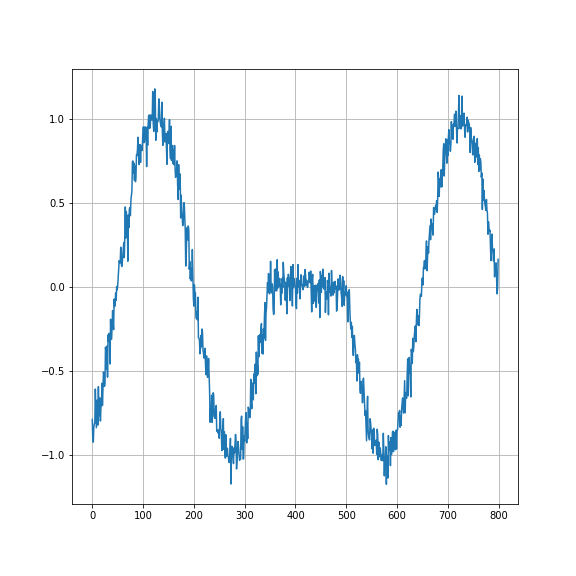
\includegraphics[height=0.3\textheight,width=0.98\textwidth]{images/intro_ood_anomaly/anomaly_train.png}
%        \caption{}
%        \label{fig:anomaly_time}
%    \end{subfigure}
%    \begin{subfigure}{0.333\textwidth}
%        \centering
%        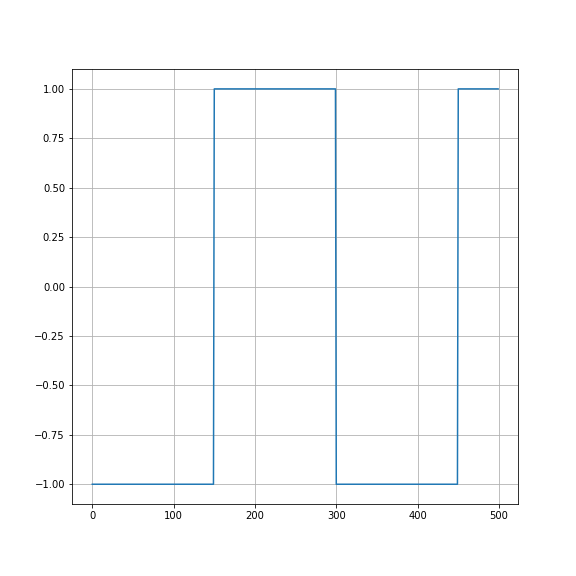
\includegraphics[height=0.3\textheight,width=0.98\textwidth]{images/intro_ood_anomaly/ood_train.png}
%        \caption{}
%        \label{fig:ood_time}
%    \end{subfigure}
%    \caption{Illustration of anomaly and OOD with time series data as example. \ref{fig:normal_train_time} depicts the triaining data as sinusoidal wave.
%    \ref{fig:anomaly_time} represents the anomaly in the sinusoidal wave and \ref{fig:ood_time} represents the square wave as OOD signal}
%\end{figure}

\end{document}
